\documentclass[12pt,letterpaper]{report}
\usepackage{pgf, tikz}
\usetikzlibrary{arrows, automata,shapes.geometric}

\begin{document}
\tikzset{elliptic state/.style={draw,ellipse}}
    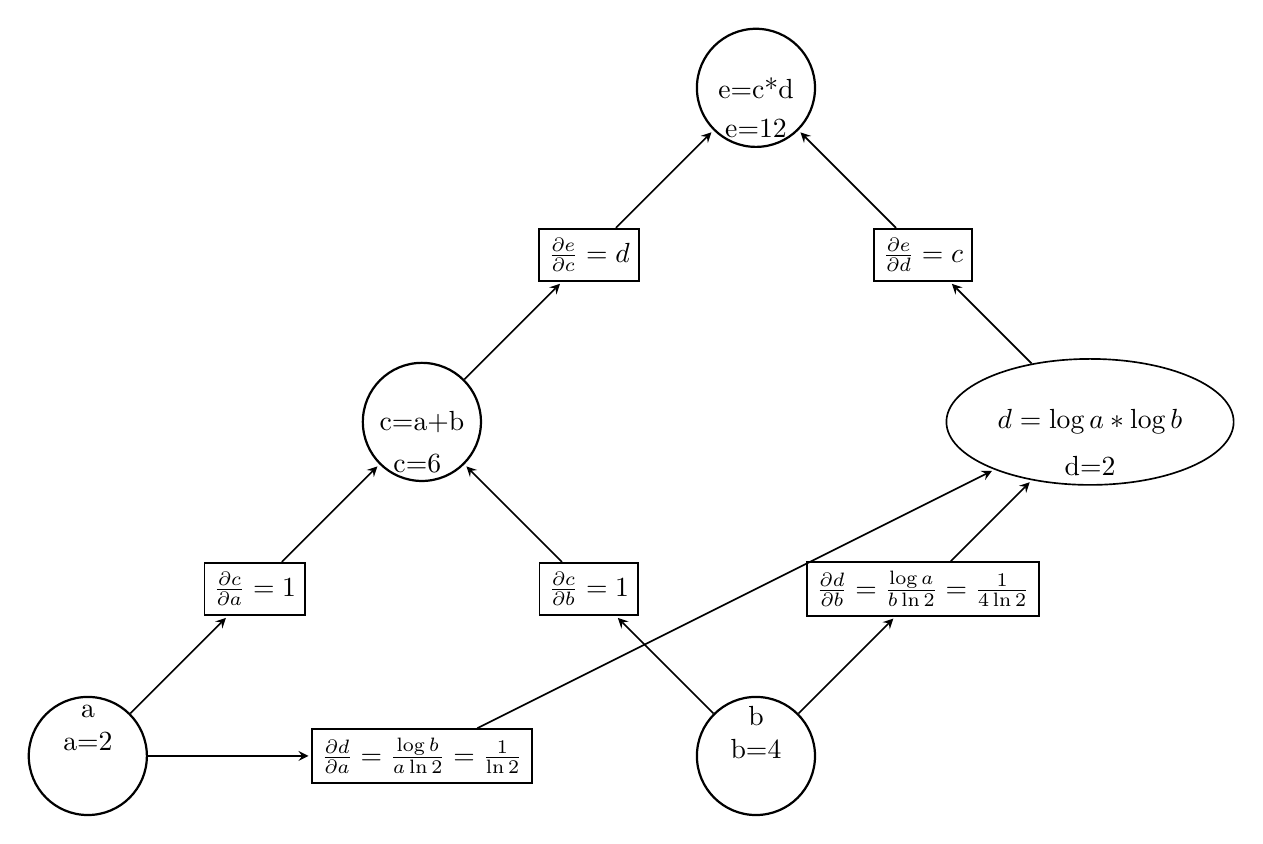
\begin{tikzpicture}[
            > = stealth, % arrow head style
            shorten > = 1pt, % don't touch arrow head to node
            auto,
            node distance = 3cm, % distance between nodes
            semithick % line style
        ]

        \tikzstyle{every state}=[
            draw = black,
            thick,
            fill = white,
            minimum size = 15mm
        ]

        \node[state] (e) {e=c*d};
        \node[align=center,anchor=south] (elabel) at (e.south) {e=12};

        \node[rectangle,draw] (ec) [below left of=e]{$\frac{\partial e}{\partial c}=d$};
        \node[rectangle,draw] (ed) [below right of=e]{$\frac{\partial e}{\partial d}=c$};
        
        \node[state] (c) [below left of=ec]{c=a+b};
        \node[align=center,anchor=south] (clabel) at (c.south) {c=6 };

        \node[draw,ellipse,minimum size=16mm] (d) [below right of=ed]{$d=\log a*\log b$};
        \node[align=center,anchor=south] (dlabel) at (d.south) {d=2};
        
        
        \node[rectangle,draw] (ca) [below left of=c]{$\frac{\partial c}{\partial a}=1$};
        \node[rectangle,draw] (cb) [below right of=c]{$\frac{\partial c}{\partial b}=1$};
        \node[state] (a) [below left of=ca]{};
        \node[align=center,anchor=north] (alabel) at (a.north) {a\\a=2};

        \node[state] (b) [below right of=cb]{};
        \node[align=center,anchor=north] (blabel) at (b.north) {b\\b=4};
        \node[rectangle,draw] (db) [below left of=d]{$\frac{\partial d}{\partial b}=\frac{\log a}{b\ln 2}=\frac{1}{4\ln 2}$};

        \node[rectangle,draw] (da) [below left of=cb]{$\frac{\partial d}{\partial a}=\frac{\log b}{a\ln 2}=\frac{1}{\ln 2}$};
        %\node[rectangle,draw] (tmp)[above of=s]{$tmp$};
        %\node[state] (v1) [above right of=s] {$v_1$};
        %\node[state] (v2) [right of=s] {$v_2$};
        %\node[state] (v3) [below right of=s] {$v_2$};
        %\node[state] (t) [right of=v2] {$t$};
        \path[->] (ec) edge (e) ;
        \path[->] (ed)  edge (e);
        \path[->]  (c) edge (ec);
        \path[->]  (ca) edge (c);
        \path[->]  (cb) edge (c);
        \path[->] (a) edge (ca);
        \path[->] (db) edge (d);
        \path[->] (b) edge (db);
        \path[->] (d) edge (ed);
        \path[->] (b) edge (cb);
        \path[->] (a) edge (da);
        \path[->] (da) edge (d);


        %\path[->] (s) edge node {18} (v1);
        %\path[->] (s) edge node {1} (v2);
        %\path[->] (s) edge node {1} (v3);
        %\path[->] (v2) edge node {2} (v1);
        %\path[->] (v3) edge node {1} (v2);
        %\path[->] (v1) edge node {20} (t);

        %\draw[red, dashed] (1, 2) -- (1, -2);
    \end{tikzpicture}

\end{document}